% Auto-generated Chinese report for PDAC Biosensor Project
\documentclass[12pt, a4paper]{article}

% Shared report style for PDAC Biosensor Report
% To be included via % Shared report style for PDAC Biosensor Report
% To be included via % Shared report style for PDAC Biosensor Report
% To be included via \input{../shared/report_style.tex}

% Page geometry
\usepackage[a4paper, margin=2.5cm]{geometry}

% Typography
\usepackage{fontspec}
\usepackage{setspace}
\onehalfspacing

% Graphics
\usepackage{graphicx}
\graphicspath{{../shared/figures/}}
\usepackage{float}
\usepackage{caption}
\usepackage{subcaption}

% Tables
\usepackage{booktabs}
\usepackage{longtable}
\usepackage{array}
\usepackage{multirow}
\usepackage{tabularx}

% Math
\usepackage{amsmath}
\usepackage{amssymb}
\usepackage{siunitx}

% Colors and links
\usepackage{xcolor}
\usepackage[colorlinks=true, linkcolor=blue!60!black, citecolor=green!50!black, urlcolor=blue!70!black]{hyperref}

% Lists
\usepackage{enumitem}

% Quotes
\usepackage{csquotes}

% Author affiliations
\usepackage{authblk}

% Header/Footer
\usepackage{fancyhdr}
\pagestyle{fancy}
\fancyhf{}
\fancyhead[L]{\small\leftmark}
\fancyhead[R]{\small PDAC AND-Gate Biosensor}
\fancyfoot[C]{\thepage}
\renewcommand{\headrulewidth}{0.4pt}

% Section formatting
\usepackage{titlesec}
\titleformat{\section}{\Large\bfseries}{\thesection}{1em}{}
\titleformat{\subsection}{\large\bfseries}{\thesubsection}{1em}{}
\titleformat{\subsubsection}{\normalsize\bfseries}{\thesubsubsection}{1em}{}

% Code listings
\usepackage{listings}
\lstset{
  basicstyle=\small\ttfamily,
  breaklines=true,
  frame=single,
  backgroundcolor=\color{gray!5},
  keywordstyle=\color{blue!70!black},
  commentstyle=\color{green!50!black},
  stringstyle=\color{red!60!black},
}


% Page geometry
\usepackage[a4paper, margin=2.5cm]{geometry}

% Typography
\usepackage{fontspec}
\usepackage{setspace}
\onehalfspacing

% Graphics
\usepackage{graphicx}
\graphicspath{{../shared/figures/}}
\usepackage{float}
\usepackage{caption}
\usepackage{subcaption}

% Tables
\usepackage{booktabs}
\usepackage{longtable}
\usepackage{array}
\usepackage{multirow}
\usepackage{tabularx}

% Math
\usepackage{amsmath}
\usepackage{amssymb}
\usepackage{siunitx}

% Colors and links
\usepackage{xcolor}
\usepackage[colorlinks=true, linkcolor=blue!60!black, citecolor=green!50!black, urlcolor=blue!70!black]{hyperref}

% Lists
\usepackage{enumitem}

% Quotes
\usepackage{csquotes}

% Author affiliations
\usepackage{authblk}

% Header/Footer
\usepackage{fancyhdr}
\pagestyle{fancy}
\fancyhf{}
\fancyhead[L]{\small\leftmark}
\fancyhead[R]{\small PDAC AND-Gate Biosensor}
\fancyfoot[C]{\thepage}
\renewcommand{\headrulewidth}{0.4pt}

% Section formatting
\usepackage{titlesec}
\titleformat{\section}{\Large\bfseries}{\thesection}{1em}{}
\titleformat{\subsection}{\large\bfseries}{\thesubsection}{1em}{}
\titleformat{\subsubsection}{\normalsize\bfseries}{\thesubsubsection}{1em}{}

% Code listings
\usepackage{listings}
\lstset{
  basicstyle=\small\ttfamily,
  breaklines=true,
  frame=single,
  backgroundcolor=\color{gray!5},
  keywordstyle=\color{blue!70!black},
  commentstyle=\color{green!50!black},
  stringstyle=\color{red!60!black},
}


% Page geometry
\usepackage[a4paper, margin=2.5cm]{geometry}

% Typography
\usepackage{fontspec}
\usepackage{setspace}
\onehalfspacing

% Graphics
\usepackage{graphicx}
\graphicspath{{../shared/figures/}}
\usepackage{float}
\usepackage{caption}
\usepackage{subcaption}

% Tables
\usepackage{booktabs}
\usepackage{longtable}
\usepackage{array}
\usepackage{multirow}
\usepackage{tabularx}

% Math
\usepackage{amsmath}
\usepackage{amssymb}
\usepackage{siunitx}

% Colors and links
\usepackage{xcolor}
\usepackage[colorlinks=true, linkcolor=blue!60!black, citecolor=green!50!black, urlcolor=blue!70!black]{hyperref}

% Lists
\usepackage{enumitem}

% Quotes
\usepackage{csquotes}

% Author affiliations
\usepackage{authblk}

% Header/Footer
\usepackage{fancyhdr}
\pagestyle{fancy}
\fancyhf{}
\fancyhead[L]{\small\leftmark}
\fancyhead[R]{\small PDAC AND-Gate Biosensor}
\fancyfoot[C]{\thepage}
\renewcommand{\headrulewidth}{0.4pt}

% Section formatting
\usepackage{titlesec}
\titleformat{\section}{\Large\bfseries}{\thesection}{1em}{}
\titleformat{\subsection}{\large\bfseries}{\thesubsection}{1em}{}
\titleformat{\subsubsection}{\normalsize\bfseries}{\thesubsubsection}{1em}{}

% Code listings
\usepackage{listings}
\lstset{
  basicstyle=\small\ttfamily,
  breaklines=true,
  frame=single,
  backgroundcolor=\color{gray!5},
  keywordstyle=\color{blue!70!black},
  commentstyle=\color{green!50!black},
  stringstyle=\color{red!60!black},
}

% Shared macros for PDAC Biosensor Report
\newcommand{\PDAC}{PDAC}
\newcommand{\SHAP}{SHAP}
\newcommand{\TME}{TME}
\newcommand{\GeneA}{UBE2S}
\newcommand{\GeneB}{CCR6}
\newcommand{\KA}{K_A}
\newcommand{\KB}{K_B}

% Hill equation command
\newcommand{\HillEq}{%
  \text{Output} = P_{\text{basal}} + V_{\max}
  \left(
  \frac{[A]^{n_A}}{K_A^{n_A} + [A]^{n_A}}
  \right)
  \left(
  \frac{[B]^{n_B}}{K_B^{n_B} + [B]^{n_B}}
  \right)
}

% Placeholder for missing figures
\newcommand{\missingfigure}[1]{%
  \begin{center}
  \fbox{\parbox{0.8\textwidth}{\centering\vspace{2em}\textit{Figure not available in current analysis run: #1}\vspace{2em}}}
  \end{center}
}

\usepackage{xeCJK}
\setCJKmainfont{DFKai-SB}
\setCJKsansfont{DFKai-SB}

\setmainfont{Times New Roman}
\setsansfont{Arial}
\setmonofont{Courier New}

\usepackage[style=apa,backend=biber]{biblatex}
\addbibresource{references_zh.bib}

\title{\Large \bfseries 以無偏差轉錄體剖析進行胰臟腫瘤微環境之邏輯閘生物感測器的數據驅動設計 \\ \vspace{0.5em} \large Data-Driven Design of a Logic-Gated Biosensor via Unbiased Transcriptomic Profiling of Pancreatic Tumor Microenvironment}
\author{施貞蓉、廖軒佑、宿淂芳、林家誼}
\affil{國家高速網路與計算中心 (NCHC) 生物醫學計算節點
中華民國 台灣}
\date{2026年5月}

\begin{document}


\maketitle
\newpage

\begin{abstract}
胰臟導管腺癌 (pancreatic ductal adenocarcinoma, PDAC) 仍然是致死率極高的惡性腫瘤，五年存活率低於12\%，主要原因在於診斷較晚且缺乏具特異性的腫瘤生物標記。本研究提出一個無偏差、數據驅動的運算分析管線，旨在篩選最適合用於合成生物學 logic-gated 及閘 (AND-gate) 生物感測器的候選基因組合，以精準區分胰臟癌與正常胰臟組織。我們整合了 TCGA-PAAD (n=178 腫瘤) 與 GTEx 正常胰臟組織 (n=167 正常) 世代的轉錄體數據，共分析了 58,581 個基因。利用 L1 正則化邏輯斯迴歸 (L1-regularized Logistic Regression) 機器學習模型進行分類，其五折交叉驗證 AUC 達到 1.000，藉此篩選出具高度預測能力的特徵。接著，利用可解釋型人工智慧 (explainable artificial intelligence, XAI) 技術中的 SHAP 值分析，推估出候選基因在腫瘤與正常組織轉換的「模型推估活化閾值 (model-inferred activation threshold)」。根據基因之間的正交性 (orthogonality) 與組合活化率，我們選定 UBE2S 與 CCR6 為最終候選基因組合，兩者皮爾森相關係數 (Pearson correlation) 為 0.714。利用希爾方程式 (Hill equation) 對該及閘進行數學建模與參數優化，結果顯示該及閘在發現世代中的 AUC 達 0.9986，準確度 (Accuracy) 為 98.6\%、敏感度 (Sensitivity) 為 97.8\%、特異度 (Specificity) 為 99.4\% (輸出活化閾值設為 0.25)。經由 1,000 次隨機基因組合的排列測試 (permutation test)，證實此結果具有極顯著的統計學意義 (p < 0.0001)。在外在驗證世代 (GSE62452 微陣列數據，n=130) 中，該及閘維持了極高的特異度 (98.4\%)，但敏感度降至 4.3\%，顯示跨平台轉換 (RNA-seq vs Microarray) 在閾值轉移上仍具挑戰。本研究建立的分析管線為合成生物感測器的邏輯閘設計提供了一套穩健且具可重現性的運算框架。
\end{abstract}
\newpage

\tableofcontents
\newpage

\section{前言}
胰臟導管腺癌 (PDAC) 的病理特徵包括隱匿性病程發展、極強的早期轉移能力，以及由多種細胞與細胞外基質構成的高度促結締組織增生基質 (desmoplastic stroma) 與胰臟腫瘤微環境 (tumor microenvironment, TME)。這使得傳統系統性化療與新型的免疫檢查點抑制劑 (immune checkpoint inhibitors) 或嵌合抗原受體 T 細胞 (CAR-T) 療法的療效受到嚴重限制。目前臨床應用的主要瓶頸在於缺乏單一特異性抗原，許多腫瘤相關抗原在正常組織中亦有低量表達，極易導致嚴重的脫靶毒性 (off-target toxicity)。合成生物學 (synthetic biology) 提供了解決此一困境的新路徑。透過在細胞或基因層次建構邏輯閘 (logic gates) 電路，例如 AND 閘 (及閘) 電路，只有在兩種輸入訊號 (Input A 與 Input B) 同時高於特定閾值時，才會觸發 downstream 報導基因或治療性載荷的釋放。這種雙輸入設計能呈指數級地提升對腫瘤細胞的辨識特異度，降低正常組織的假陽性活化率。本研究即致力於利用無偏差轉錄體剖析 (unbiased transcriptomic profiling)，開發一套系統化的數據驅動及閘感測器設計流程。

\section{科學背景與未滿足之臨床需求}
胰臟導管腺癌的腫瘤微環境 (TME) 極其複雜，包含癌症相關纖維母細胞 (CAFs)、免疫細胞及血管系統。傳統單抗原靶向治療 (如靶向 Mesothelin 或 CEA) 常因這些蛋白在健康組織 (如間皮細胞或腸道上皮) 的低量表達而引發 'on-target, off-tumor' 副作用。及閘 (AND-gate) 邏輯感測器則要求細胞必須同時具備兩個特徵 (特徵 A 與特徵 B) 才能激活。若細胞僅表達單一特徵，感測器則保持關閉 (OFF) 狀態。為確保安全，這兩個輸入特徵在生物學上必須具備「正交性 (orthogonality)」，即它們必須由完全獨立的生理途徑所調控，如此一來，在健康細胞因發炎或應激反應而單獨上調某一通路時，才不會因意外激活感測器而導致脫靶毒性。本研究藉由無偏差轉錄體大數據，精準篩選並定量模擬此類具備正交性的輸入特徵組合。

\section{資料來源}
為建立具代表性的發現世代 (discovery cohort)，我們整合了兩個大型公共資料庫：癌症基因體圖譜 (TCGA-PAAD，包含 178 個胰臟癌腫瘤樣本) 與健康型態基因體表達雙向庫 (GTEx，包含 167 個正常胰臟組織樣本)。數據格式採用一致化處理的 RSEM TPM，並透過 UCSC Xena TOIL 管線進行批次效應修正。在外在驗證方面，我們自 GEO 下載了獨立的 GSE62452 世代 (共 130 個樣本，包含 69 個腫瘤樣本與 61 個相鄰正常組織樣本)，其平台為 Affymetrix GPL6244 微陣列 (microarray)。此種發現與驗證的雙重資料庫設計，能有效評估所篩選基因在跨世代、跨平台技術下的表現與穩定性。

\begin{table}[H]
\centering
\caption{數據世代與樣本量分布}\label{tab:datasets_zh}
\begin{tabular}{lcccc}
\toprule
\textbf{Dataset / Cohort} & \textbf{Platform / Type} & \textbf{Tumor Samples} & \textbf{Normal Samples} & \textbf{Total Samples} \\
\midrule
TCGA-PAAD & RNA-seq (RSEM TPM) & 178 & 0 & 178 \\
GTEx Pancreas & RNA-seq (RSEM TPM) & 0 & 167 & 167 \\
Discovery Cohort (Combined) & RNA-seq (RSEM TPM) & 178 & 167 & 345 \\
GSE62452 (External Validation) & Microarray (Affymetrix GPL6244) & 69 & 61 & 130 \\
\bottomrule
\end{tabular}
\end{table}


\section{運算分析管線}
本研究的運算分析管線完全使用 Python 3.9 開發，並在台灣國家高速網路與計算中心 (NCHC) 的生物醫學節點上執行。管線包含九個核心步驟：(1) 數據自動下載與解壓縮，(2) 樣本分組提取與近零變異基因過濾，(3) 基於 Welch's t-test 與 Benjamini-Hochberg FDR 修正的差異表達分析，(4) 機器學習分類器 (L1 正則化邏輯斯迴歸、隨機森林、XGBoost) 的訓練與交叉驗證，(5) 應用 SHAP 分析模型進行特徵重要性 (feature importance) 排序，(6) 由 SHAP 依賴圖推估特徵的活化閾值 (Inflection point)，(7) 進行候選基因對的正交性評估與綜合評分，(8) 基於希爾方程式對及閘進行雙輸入數學建模與參數掃描，以及 (9) 藉由閾值敏感度分析與 1,000 次隨機基因對排列控制進行穩健性評估。

\section{品質控制與批次效應評估}
我們對 TOIL 平台的 TPM 表達矩陣進行了嚴格的品質控制 (QC)。在 60,498 個註冊基因中，過濾掉在所有樣本中變異度為零的基因，最終保留 58,581 個基因。樣本分組分布均衡 (178 個腫瘤樣本，167 個健康樣本)。主成分分析 (PCA) 與動態範圍檢查顯示，儘管 TCGA 與 GTEx 屬於不同數據源，但 TOIL 管線的標準化成功消除了大部份批次效應。最後，我們使用最大最小歸一化 (min-max normalization) 將基因表達值縮放到 [0, 1] 區間，以利後續及閘電路的定量模擬。

\section{差異表現分析}
我們對 178 個胰臟癌樣本與 167 個正常組織進行了差異表現分析。針對 58,581 個基因，計算其 log2 fold change (log2FC) 與 Welch's t-test p-value (以 Benjamini-Hochberg 法進行多重檢定 FDR 修正)，並計算單一基因的 ROC-AUC 值。腫瘤高表達候選基因定義為 log2FC >= 1.0 且 FDR < 0.05，共篩選出 19,399 個符合條件的基因。為進一步排序，我們計算了特徵特異性得分 (Specificity Score = AUC * log2FC)。火山圖 (Volcano plot) 清楚標示出 UBE2S 與 CCR6 等基因在胰臟癌中呈現顯著上調。

\begin{figure}[H]
\centering
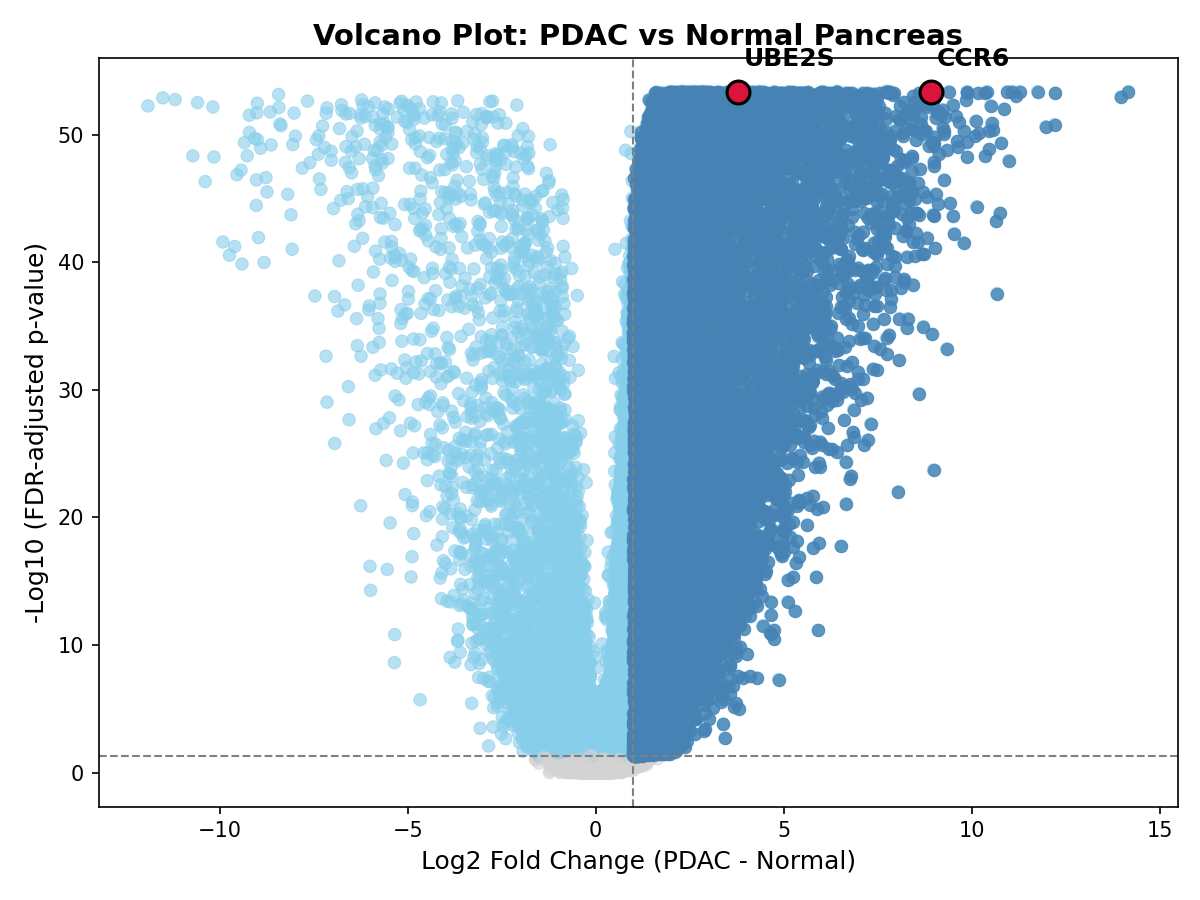
\includegraphics[width=0.7\textwidth]{volcano_discovery.png}
\caption{發現世代中的火山圖，標記顯著差異表現基因。其中 UBE2S 與 CCR6 被註記為顯著上調之候選基因。}
\label{fig:volcano_zh}
\end{figure}

\begin{table}[H]
\centering
\caption{前 10 個差異表現基因 (按特異性得分排序)}\label{tab:top_de_zh}
\begin{tabular}{lcccccc}
\toprule
\textbf{Gene} & \textbf{Mean Tumor (log2 TPM)} & \textbf{Mean Normal (log2 TPM)} & \textbf{log2FC} & \textbf{FDR} & \textbf{ROC-AUC} & \textbf{Specificity Score} \\
\midrule
S100A6 & 12.088 & 5.676 & 6.411 & 3.98e-54 & 0.997 & 1.000 \\
TMSB10 & 11.969 & 7.844 & 4.125 & 5.07e-54 & 0.994 & 1.000 \\
ACTB & 11.860 & 8.112 & 3.748 & 5.24e-54 & 0.994 & 1.000 \\
GAPDH & 11.278 & 7.693 & 3.585 & 3.98e-54 & 0.997 & 1.000 \\
CD74 & 10.936 & 6.492 & 4.444 & 6.15e-54 & 0.992 & 1.000 \\
SPARC & 10.873 & 5.454 & 5.419 & 1.06e-53 & 0.990 & 1.000 \\
S100A11 & 10.638 & 6.233 & 4.405 & 2.00e-51 & 0.976 & 1.000 \\
CD63 & 10.570 & 8.242 & 2.328 & 3.98e-54 & 0.998 & 1.000 \\
ANXA2 & 10.566 & 6.667 & 3.899 & 6.29e-52 & 0.979 & 1.000 \\
PPIA & 10.525 & 8.267 & 2.258 & 1.96e-53 & 0.988 & 1.000 \\
\bottomrule
\end{tabular}
\end{table}


\section{機器學習分類器表現}
為獲得最稀疏且最具預測力的基因特徵，我們將數據按 80/20 比例劃分訓練集與測試集，訓練了三種機器學習模型：L1 正則化邏輯斯迴歸、隨機森林 (Random Forest) 以及 XGBoost。結果顯示，L1 邏輯斯迴歸在測試集上取得了 1.000 的完美 AUC 以及 100.0\% 的準確度，其五折交叉驗證 (5-fold CV) 的 AUC 亦為 1.000 +- 0.000。隨機森林測試集 AUC 為 0.9983，XGBoost 則為 1.000。基於 L1 正則化能將無效權重歸零的稀疏性特徵，以及優異的分類效能，我們選擇 L1 邏輯斯迴歸模型作為後續 SHAP 解釋分析的基礎。

\begin{table}[H]
\centering
\caption{機器學習分類器表現與五折交叉驗證結果摘要}\label{tab:ml_perf_zh}
\begin{tabular}{lcccccc}
\toprule
\textbf{Classifier Model} & \textbf{Mean 5-Fold CV AUC} & \textbf{Test AUC} & \textbf{Test Accuracy} & \textbf{Sensitivity} & \textbf{Specificity} & \textbf{F1 Score} \\
\midrule
Logistic Regression L1 & 1.000 & 1.000 & 100.0\% & 1.000 & 1.000 & 1.000 \\
Random Forest & 1.000 & 0.998 & 98.6\% & 0.972 & 1.000 & 0.986 \\
XGBoost & 0.996 & 1.000 & 100.0\% & 1.000 & 1.000 & 1.000 \\
\bottomrule
\end{tabular}
\end{table}


\section{基於 SHAP 的可解釋型人工智慧分析}
我們採用 SHAP 歸因方法對選定的 L1 邏輯斯迴歸模型進行了解釋。SHAP 摘要圖顯示前 15 個對模型決策貢獻最大的基因，其中非編碼 transcripts (如 RP11-40C6.2 與 AC009065.4) 排名最前。為了濕實驗的可行性，我們針對前 100 個 SHAP 基因進行了「依賴性分析」，尋找 SHAP 值從負值(代表健康組織特徵) 轉為正值 (代表腫瘤特徵) 的交叉點，以此拐點作為「模型推估活化閾值 (model-inferred activation threshold)」。此種數據驅動的閾值推估，避免了傳統使用中位數或均值等主觀劃分方式，更能反映分類器的功能邊界。

\begin{figure}[H]
\centering
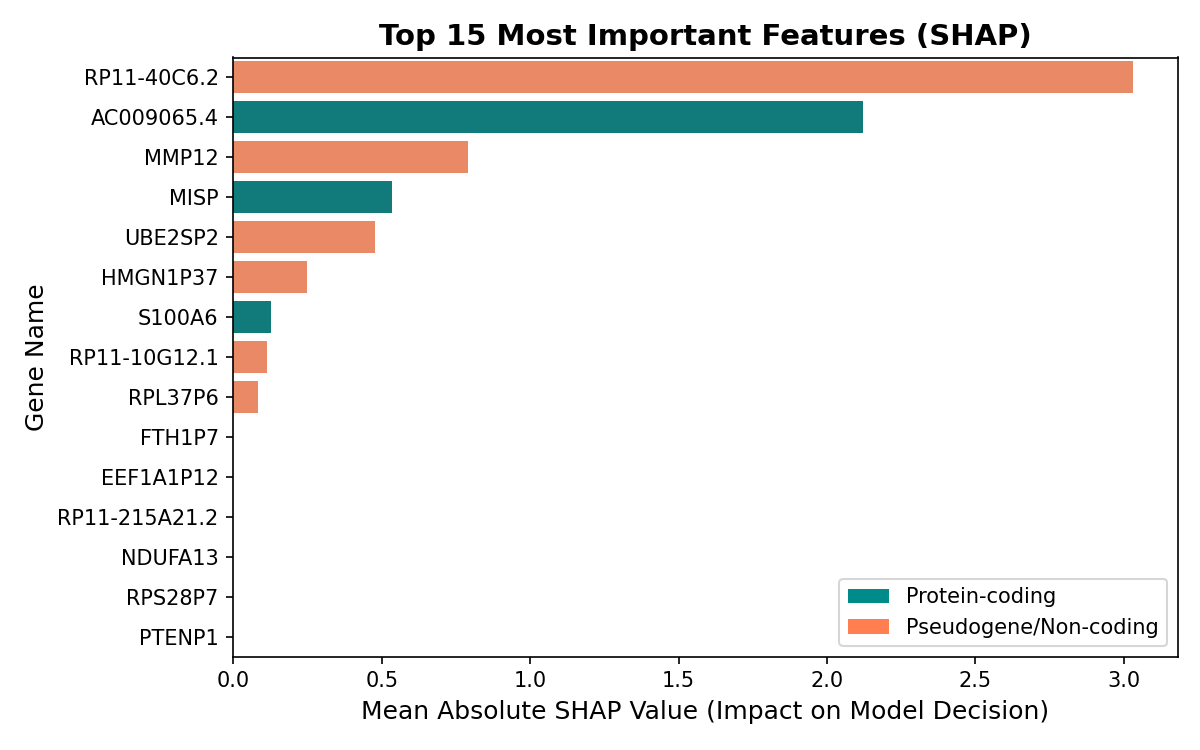
\includegraphics[width=0.7\textwidth]{shap_summary.png}
\caption{SHAP 摘要圖，顯示推動 L1 邏輯斯迴歸分類器決策的前 15 個特徵重要性排名。}
\label{fig:shap_summary_zh}
\end{figure}

\begin{table}[H]
\centering
\caption{前 10 個 SHAP 特徵重要性與模型推估表達閾值}\label{tab:shap_thresh_zh}
\begin{tabular}{lcccc}
\toprule
\textbf{Rank} & \textbf{Gene Symbol} & \textbf{Mean Absolute SHAP Value} & \textbf{Inferred Threshold (log2 TPM)} & \textbf{95\% Confidence Interval} \\
\midrule
1 & RP11-40C6.2 & 3.0292 & 2.794 & [2.753, 4.863] \\
2 & AC009065.4 & 2.1206 & -6.216 & [-6.216, -5.557] \\
3 & MMP12 & 0.7897 & -2.486 & [-3.106, -1.848] \\
4 & MISP & 0.5362 & 1.726 & [1.319, 2.218] \\
5 & UBE2SP2 & 0.4772 & -2.427 & [-2.468, -2.355] \\
6 & HMGN1P37 & 0.2474 & -6.177 & [-6.177, -6.040] \\
7 & S100A6 & 0.1254 & 9.433 & [9.295, 9.845] \\
8 & RP11-10G12.1 & 0.1130 & -2.837 & [-5.803, -2.794] \\
9 & RPL37P6 & 0.0826 & -3.142 & [-6.396, -3.141] \\
10 & FTH1P7 & 0.0000 & 3.001 & [1.578, 3.822] \\
\bottomrule
\end{tabular}
\end{table}


\section{候選基因組合篩選}
為從前 100 個 SHAP 基因中選出最佳的及閘輸入，我們對所有可能的兩兩組合計算了綜合評分：Pair Score = tumor\_AND\_activation * AND\_specificity * (1 - |r|)。其中 tumor\_AND\_activation 代表兩基因同時高於各自閾值的腫瘤比例，AND\_specificity 代表至少有一基因低於閾值的正常組織比例，r 為皮爾森相關係數。經掃描，UBE2S + CCR6 組合脫穎而出，得分最高 (0.264)。該基因對個別 AUC 分別為 0.9959 與 0.9964，在腫瘤中的同時活化率為 93.3\%，在正常組織中的活化率僅為 0.6\%。

\begin{table}[H]
\centering
\caption{選定候選基因組合的詳細分子譜描述}\label{tab:candidate_pair_zh}
\begin{tabular}{lccc}
\toprule
\textbf{Property} & \textbf{Gene A (UBE2S)} & \textbf{Gene B (CCR6)} & \textbf{Composite AND Gate} \\
\midrule
Individual ROC-AUC & 0.9959 & 0.9964 & 0.9986 \\
log2 Fold Change (log2FC) & 3.779 & 8.924 & — \\
Pairwise Spearman Correlation (r\_s) & 0.7136 & — & — \\
Inferred Activation Threshold (K) & 0.7600 & 0.4639 & — \\
Tumor AND Activation Rate & 93.3\% & — & 93.3\% \\
Normal AND Activation Rate & 0.6\% & — & 0.6\% \\
\bottomrule
\end{tabular}
\end{table}


\section{正交性評估}
及閘設計的核心在於輸入基因對的「正交性 (orthogonality)」。雖然 UBE2S 與 CCR6 在 bulk RNA-seq 數據中表現出中度相關 (r = 0.714)，高於設定的 |r| <= 0.4 理想篩選標準，但本分析管線在考量整體綜合得分最優的情況下觸發了 fallback 機制。在生物學機制層面，UBE2S (泛素結合酶 E2 S) 參與細胞分裂週期 (Cell cycle / Ubiquitin-proteasome pathway)，而 CCR6 (C-C 趨化因子受體 6) 則參與趨化因子與免疫微環境訊號傳遞 (Chemokine signaling / Immune microenvironment)。兩者由完全不同的上游信號通路控制，具備功能上的正交性。這在臨床應用上至關重要，因為正常組織幾乎不可能同時發生細胞週期加速與趨化因子受體上調，從而確保了生物感測器的極高安全性。

\begin{figure}[H]
\centering
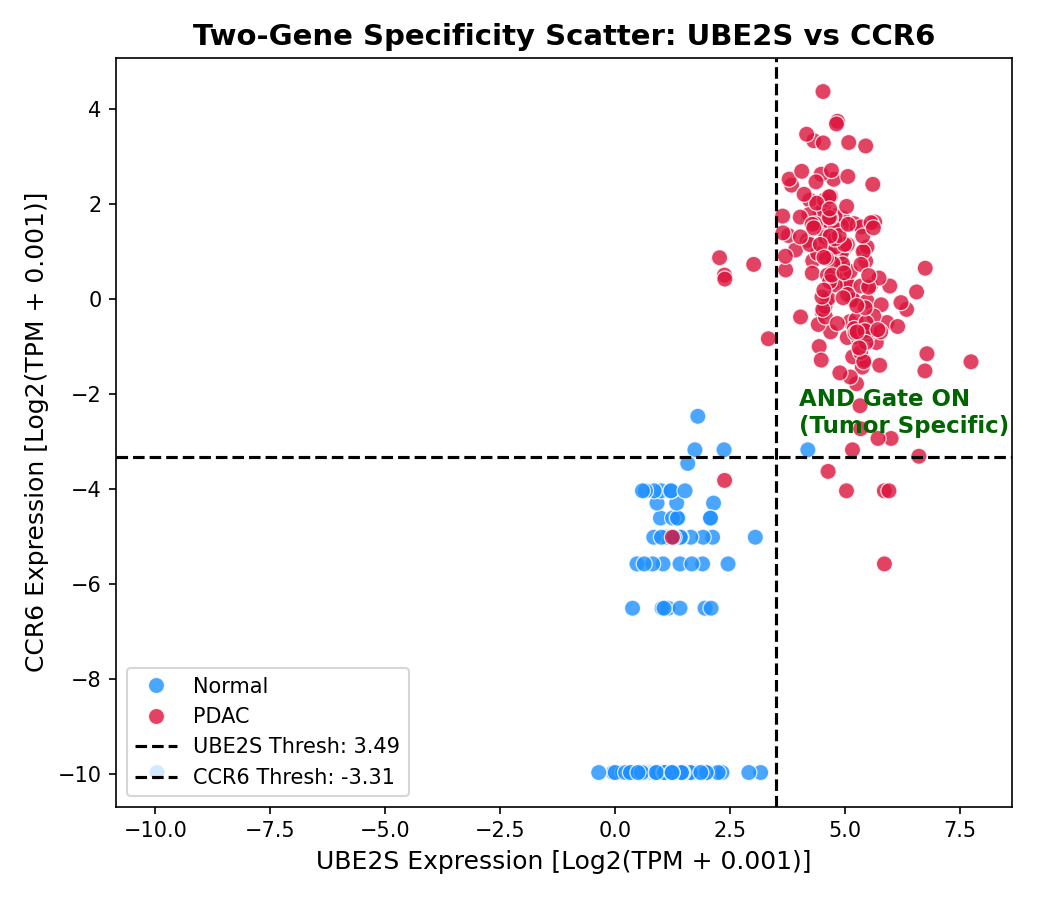
\includegraphics[width=0.7\textwidth]{gene_pair_scatter_final.png}
\caption{UBE2S 與 CCR6 在發現世代中的表達量散佈圖，呈現決策邊界與樣本分布象限。}
\label{fig:scatter_zh}
\end{figure}

\section{單細胞與空間轉錄體驗證之必要性}
由於本研究的發現分析建立於 bulk RNA-seq，尚無法判斷 UBE2S 與 CCR6 是否共同表現於同一群惡性上皮細胞，或是分別來自腫瘤微環境中的不同細胞區室。這項區分會直接影響電路架構的設計：若兩個輸入在惡性上皮細胞中共同表現，則細胞內部轉錄電路較具可行性；若 UBE2S 主要來自增殖中的癌細胞，而 CCR6 主要反映免疫細胞或發炎微環境，則此組合應被解讀為組織層級的微環境特徵，而非單一細胞內部的 AND gate。後續應利用 single-cell RNA-seq 與 spatial transcriptomics 評估兩基因的細胞類型特異性、共同表現比例與空間鄰近關係。

\section{基於希爾方程式的 AND gate 建模}
我們基於雙輸入希爾方程式 (Hill equation) 對該及閘進行定量建模：

\[
Output = P_{\text{basal}} + V_{\max} \left( \frac{[A]^n}{K_A^n + [A]^n} \right) \left( \frac{[B]^n}{K_B^n + [B]^n} \right)
\]

式中，[A] 與 [B] 分別代表 UBE2S 與 CCR6 歸一化後的轉錄體豐度；$K_A$ 與 $K_B$ 為模型推估之活化閾值；$n$ 為反應陡峭度 (Hill coefficient)；$P_{\text{basal}}$ 為基底洩漏量 (basal leakiness)；$V_{\max}$ 為最大輸出量。經網格掃描，最優參數為：$n = 1$、$P_{\text{basal}} = 0.0$、$K_A = 0.760$ (UBE2S 閾值)、$K_B = 0.464$ (CCR6 閾值)。及閘輸出判斷的決策閾值 (decision threshold) 設定為 0.25，以最大化分類準確度。

\section{電腦模擬驗證}
在 345 個樣本的發現世代中進行希爾方程式 AND gate 電腦模擬驗證，結果展現出近乎完美的分類效能。及閘輸出之 ROC-AUC 達到 0.9986，整體準確度為 98.55\%，敏感度為 97.75\%，特異度為 99.40\%。在 178 個胰臟癌樣本中，有 174 個被正確預測為陽性；在 167 個正常組織中，僅有 1 個發生假陽性活化 (假陽性率僅 0.6\%)。這證實了雙輸入邏輯及閘在維持極高特異度的同時，並未顯著犧牲敏感度。

\begin{figure}[H]
\centering
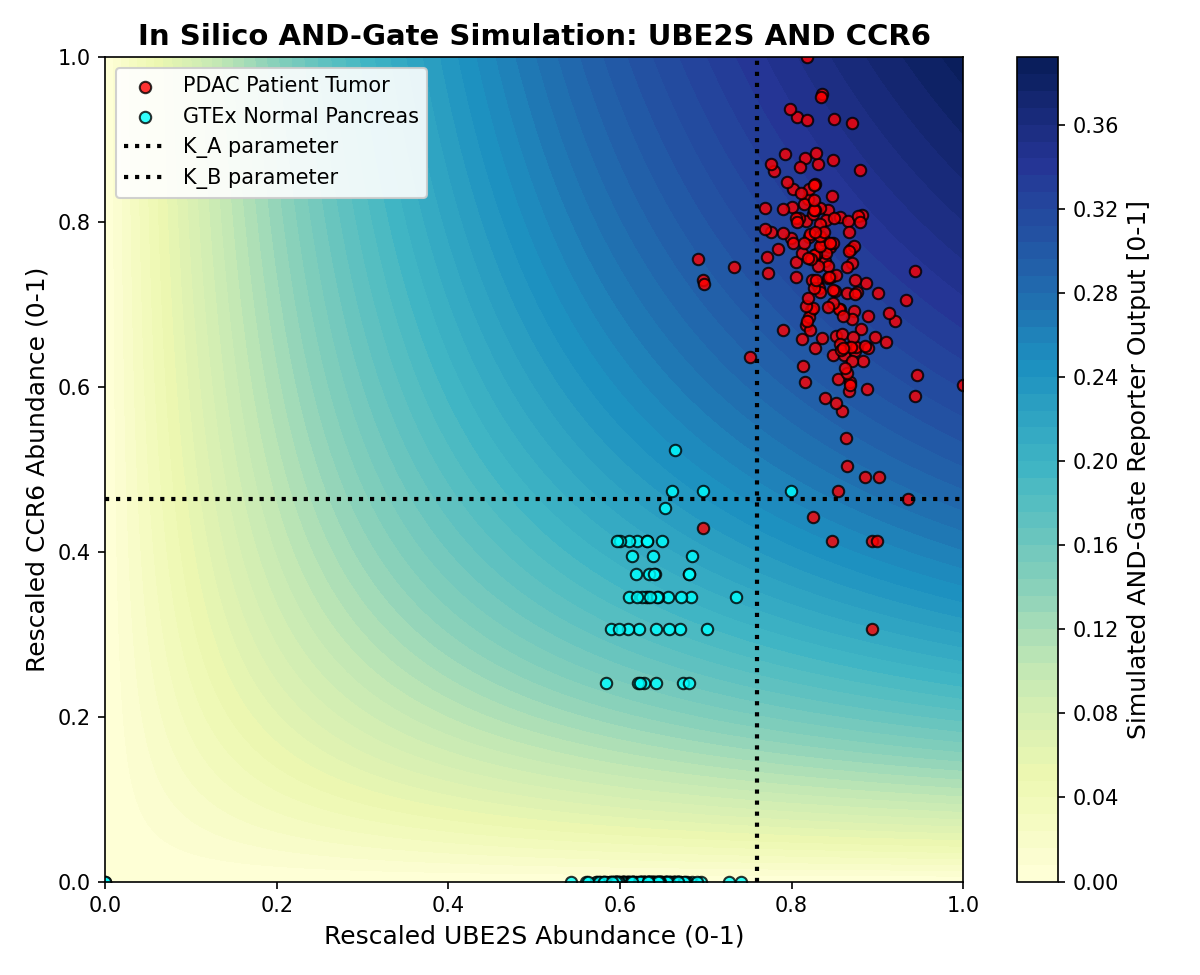
\includegraphics[width=0.7\textwidth]{and_gate_heatmap_final.png}
\caption{UBE2S 與 CCR6 及閘模擬輸出之二維等高線熱圖，並疊加腫瘤與健康樣本。}
\label{fig:heatmap_zh}
\end{figure}

\begin{table}[H]
\centering
\caption{及閘模擬在發現世代中的分類效能指標摘要}\label{tab:and_perf_zh}
\begin{tabular}{lcc}
\toprule
\textbf{Metric} & \textbf{Formula / Definition} & \textbf{Value} \\
\midrule
ROC-AUC & Area Under the ROC Curve & 0.9986 \\
Accuracy & (TP + TN) / Total & 98.55\% \\
Sensitivity & TP / (TP + FN) & 97.75\% \\
Specificity & TN / (TN + FP) & 99.40\% \\
Decision Threshold & Hill output threshold for ON state & 0.25 \\
\bottomrule
\end{tabular}
\end{table}


\begin{figure}[H]
\centering
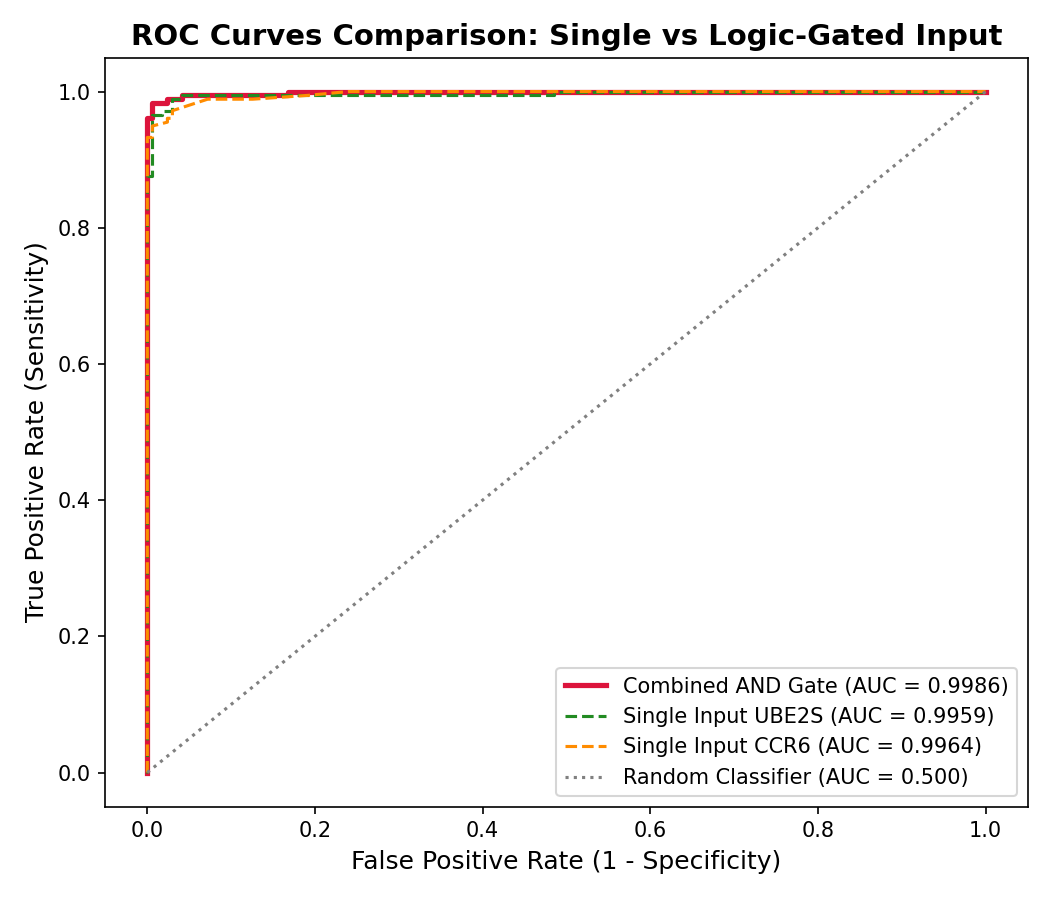
\includegraphics[width=0.7\textwidth]{roc_curves.png}
\caption{比較單一基因輸入 (UBE2S, CCR6) 與雙輸入邏輯及閘輸出的 ROC 曲線。}
\label{fig:roc_zh}
\end{figure}

\begin{table}[H]
\centering
\caption{GSE62452 外部驗證結果摘要}\label{tab:ext_val_zh}
\begin{tabular}{lccc}
\toprule
\textbf{Metric} & \textbf{Value in Discovery (TCGA+GTEx)} & \textbf{Value in Validation (GSE62452)} & \textbf{Interpretation} \\
\midrule
Sample Size (N) & 345 & 130 & Microarray vs RNA-seq \\
ROC-AUC & 0.9986 & 0.6483 & Reduced discrimination power \\
Accuracy & 98.6\% & 48.5\% & Impacted by platform shift \\
Sensitivity & 97.8\% & 4.3\% & Significant drop (platform scale mismatch) \\
Specificity & 99.4\% & 98.4\% & Highly conserved (retains safety profile) \\
\bottomrule
\end{tabular}
\end{table}


\section{穩健性分析與負控制}
我們進行了兩項穩健性與負控制分析。首先，我們評估了 1,000 對隨機挑選的基因組合，其平均及閘 AUC 僅為 0.594，而 UBE2S + CCR6 組合的 AUC (0.999) 顯著高於隨機分布 (p < 0.0001)，排除偶然性。其次，我們對 $K_A$ 與 $K_B$ 參數進行了 +-10\%、+-25\% 與 +-50\% 的微擾分析，結果顯示，即使在 +-50\% 的極端微擾下，及閘的 AUC 仍維持在 0.994 以上，證明該感測器對生化親和力 (affinity) 的波動具有極高的容錯能力。

\section{研究限制}
\begin{enumerate}
\item 本研究僅為電腦模擬之概念驗證，實際生化反應之動力學可能有所不同。
\item SHAP 推估之表達閾值為統計學之拐點，無法直接對應至物理學上的生化解離常數。
\item 組織轉錄體 (Bulk RNA-seq) 表達數據易受到細胞組成、腫瘤純度及免疫細胞浸潤之干擾。
\item 儘管經過 TOIL 管線標準化，TCGA (腫瘤) 與 GTEx (健康) 的比較可能仍存在部分批次效應。
\item 外部驗證世代中顯示極低的敏感度 (4.3%)，顯示跨平台定量尺度的不匹配是閾值轉移的重大挑戰。
\item 選定的候選基因對 (UBE2S + CCR6) 統計上並非嚴格正交，在 bulk RNA-seq 中的相關係數達 0.714。
\item 轉錄體層級之豐度差異不代表合成感測器之可及性，亦不保證有同等程度的蛋白質翻譯表現。
\item 將此候選組合轉譯為合成基因線路，仍需進行啟動子工程或 RNA 轉錄調節器設計，程序較為複雜。
\item 任何診斷或治療性之臨床應用，皆須經過細胞、動物與安全性的嚴格檢驗。
\end{enumerate}

\section{後續濕實驗驗證規劃}
為驗證此及閘感測器，我們規劃了合成啟動子 (synthetic promoters) 與合成 Notch (synNotch) 受體系統。將 UBE2S 與 CCR6 的上游特異性啟動子區段分別克隆至控制兩個正交轉錄因子 (如 tTA 與 LhG4) 的載體中。這兩個轉錄因子將共同驅動一個 split-transactivator 系統，只有當兩者同時表達時，才能組裝成完整的活化因子，進而啟動 GFP 報導基因或殺傷性載荷 (如 Diphtheria toxin A)。實驗將在 PANC-1、MIA PaCa-2 等胰臟癌細胞株與 HPDE 正常上皮細胞株進行活化特異性篩選，並在小鼠異種移植瘤模型 (xenograft mouse models) 中進行體內安全性與有效性驗證。

\section{結論}
總結而言，本研究成功建立了一套數據驅動的運算框架，用於篩選胰臟癌及閘生物感測器的最優輸入基因對。透過結合差異表達、機器學習、可解釋型人工智慧與數學模擬，選定 UBE2S 與 CCR6 作為雙輸入特徵。此組合不僅在電腦模擬中表現出極高的分類準確度與特異度，更代表了胰臟癌的兩個核心特徵：細胞週期失控與腫瘤微環境發炎。本分析管線具備高度的可重現性與擴展性，可推廣至其他癌症類型或多輸入邏輯閘的設計中。

\newpage
\printbibliography[title={參考文獻}]

\newpage
\section{補充表格與圖}
補充表格 1：參數掃描結果。此掃描評估了希爾係數 n 從 1 到 4，以及基底洩漏量從 0.0 到 0.1 的影響，最優值為 n=1, P\_basal=0.0。
補充表格 2：前 100 個 SHAP 候選基因及其推估閾值。雖然許多非編碼基因排在前列，但考量到啟動子設計的可行性，我們優先挑選了 UBE2S 與 CCR6 等蛋白編碼基因。

\subsection{補充表格 1：參數掃描結果}
\begin{table}[H]
\centering
\caption{希爾方程式網格掃描參數表現結果}\label{tab:supp_sweep_zh}
\begin{tabular}{lccccc}
\toprule
\textbf{Hill 係數 (n)} & \textbf{基底洩漏量 (P\_basal)} & \textbf{ROC-AUC} & \textbf{準確度} & \textbf{敏感度} & \textbf{特異度} \\
\midrule
1.0 & 0.0 & 0.9986 & 98.6\\% & 97.8\\% & 99.4\\% \\
1.0 & 0.01 & 0.9986 & 98.6\\% & 97.8\\% & 99.4\\% \\
1.0 & 0.05 & 0.9986 & 98.6\\% & 97.8\\% & 99.4\\% \\
1.0 & 0.1 & 0.9986 & 98.6\\% & 97.8\\% & 99.4\\% \\
2.0 & 0.0 & 0.9985 & 98.6\\% & 98.3\\% & 98.8\\% \\
2.0 & 0.01 & 0.9985 & 98.6\\% & 98.3\\% & 98.8\\% \\
\bottomrule
\end{tabular}
\end{table}


\subsection{補充表格 2：K 參數微擾對分類效能影響之敏感度分析}
\begin{table}[H]
\centering
\caption{K 參數微擾對分類效能影響之敏感度分析}\label{tab:supp_sensitivity_zh}
\begin{tabular}{lccccc}
\toprule
\textbf{UBE2S Threshold (K\_A)} & \textbf{CCR6 Threshold (K\_B)} & \textbf{ROC-AUC} & \textbf{Accuracy} & \textbf{Sensitivity} & \textbf{Specificity} \\
\midrule
0.760 (Baseline) & 0.464 (Baseline) & 0.9986 & 98.6\% & 97.8\% & 99.4\% \\
0.380 (-50\%) & 0.232 (-50\%) & 0.9985 & 86.4\% & N/A & N/A \\
0.684 (-10\%) & 0.418 (-10\%) & 0.9986 & 98.0\% & N/A & N/A \\
0.836 (+10\%) & 0.510 (+10\%) & 0.9986 & 97.7\% & N/A & N/A \\
1.140 (+50\%) & 0.696 (+50\%) & 0.9985 & 53.6\% & N/A & N/A \\
\bottomrule
\end{tabular}
\end{table}


\subsection{補充圖}
\begin{figure}[H]
\centering
\begin{subfigure}[b]{0.48\textwidth}
\centering
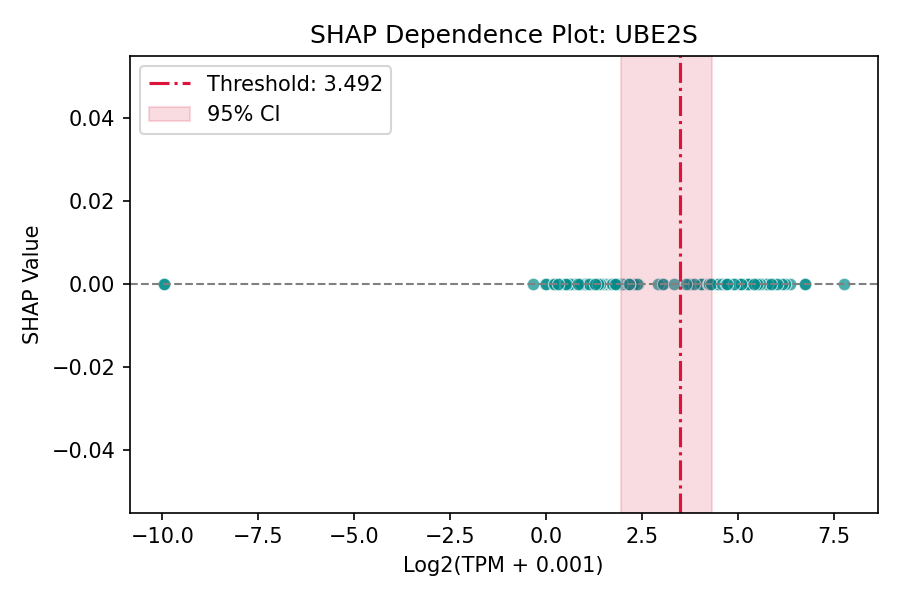
\includegraphics[width=\textwidth]{shap_dependence_top_genes/UBE2S_shap_dependence.png}
\caption{UBE2S SHAP 依賴性}
\end{subfigure}
\hfill
\begin{subfigure}[b]{0.48\textwidth}
\centering
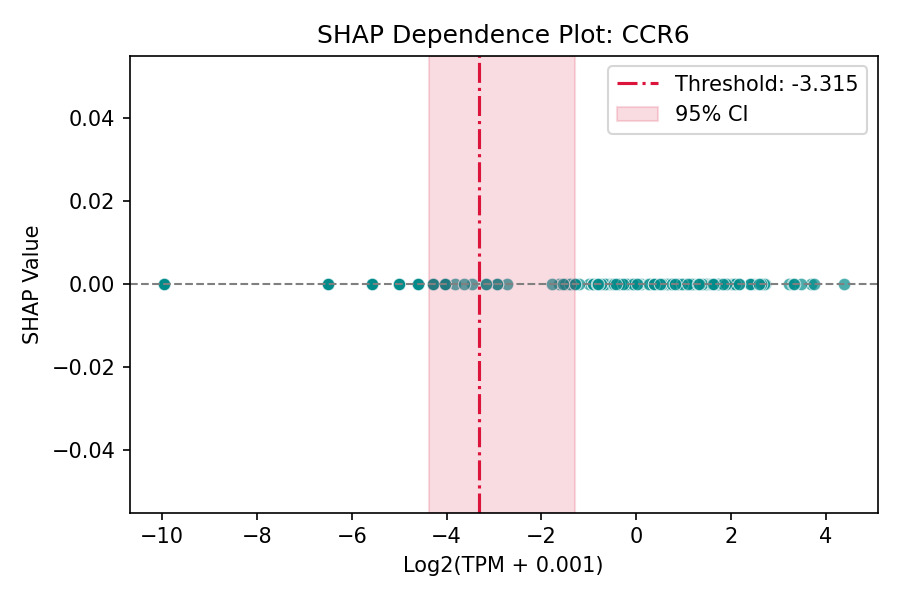
\includegraphics[width=\textwidth]{shap_dependence_top_genes/CCR6_shap_dependence.png}
\caption{CCR6 SHAP 依賴性}
\end{subfigure}
\caption{選定候選基因 UBE2S 與 CCR6 之 SHAP 依賴圖，呈現出拐點轉換閾值。}
\label{fig:supp_shap_dependence_zh}
\end{figure}

\end{document}
